\documentclass{book}

\usepackage{setspace}
\usepackage{paralist}
\usepackage{multicol} %% Useful
\usepackage{hyperref}
\usepackage{shapepar}
\usepackage{amssymb}
\usepackage{breqn}
\usepackage{amsfonts}
\usepackage{subfigure}
\usepackage{amsmath, amsthm}
\usepackage{caption}
\usepackage{xepersian}

\settextfont{Traditional Arabic}
\setcounter{tocdepth}{4}
\setcounter{secnumdepth}{4}
\setdigitfont{Traditional Arabic}

\newtheorem{thm}{قضیه}[chapter]
\newtheorem{Def}{تعریف}[section]

\newcommand{\dd}{\, \mathrm{d}}
\newcommand{\mian}[2]{\frac{#1_1 + #1_2 + \dots + #1_{#2}}{n}}

\defpersianfont\BNaz{B NAZANIN.TTF}
\deflatinfont\Time{TIMES.TTF}

\huge{\title{\lr{$4th$ $File$}}}
\author{علی}

\begin{document}
	\maketitle
	%...
	%\doublespacing
	\tableofcontents
	\singlespacing
	%...
	\Time
\chapter{\lr{$tables$}}	
\BNaz
بررسی ساختن جدول:
\begin{table}[h!]

\begin{center}
 \begin{tabular}{|c|r|p{2cm}||l|}
	\hline
	ردیف &
	\textbf{نام} &
	\centering
	 نام خانوادگی & قد \\
	\hline
	&
شماره تماس &
\centering
 رشته & تاهل\\
	\hline
 \end{tabular}
\end{center}
\caption{استخدام}
\label{Tab1}
\end{table}
\\
	در جدول \ref{Tab1} دیدیم که ...
	
\begin{table}[h!]
	\begin{center}
		\begin{tabular}{|c|c|r|}
			\hline
			&
			\multicolumn{2}{|l|}{مشخصات فردی} \\
			\cline{1-3}

نام & نام خانوادگی & مقطع تحصیلی 
\\
\hline
\multicolumn{2}{|c|}{آزمایش} 
&
دی ان ای \\
\hline
		\end{tabular}
	\end{center}
\caption{چند ستونه}
\label{Tab2}
\end{table}
در جدول \ref{Tab2}
ما شاهدیم که .....
\chapter{\lr{$Pictures$ $Figures$}}
\section{Figures}
چگونه عکس را به لاتک ضمیمه کنیم؟
\begin{figure}[h!]
	\caption*{text...}
	\begin{center}
		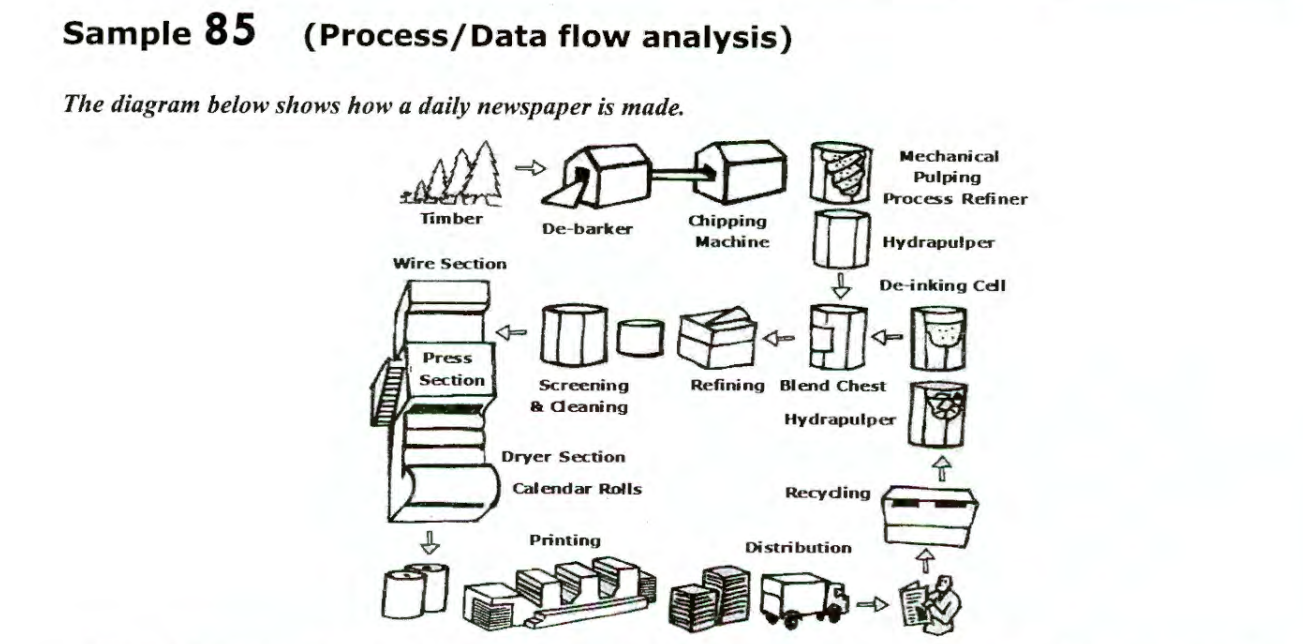
\includegraphics[width=8cm, height=5cm]{Capture.PNG}
	\end{center}
\caption{\lr{IELTS Writing Task 1}}
\label{Fig1}
\end{figure}

متن بعد از عکس ما، عکس \ref{Fig1}
که برای آزمون زبان اینگلیسی بین المللی است.
\\

\section{MultiFigures}
ساختار چند عکسی...
\begin{figure}[h!]
	\begin{center}
		\subfigure[Moscow]{
		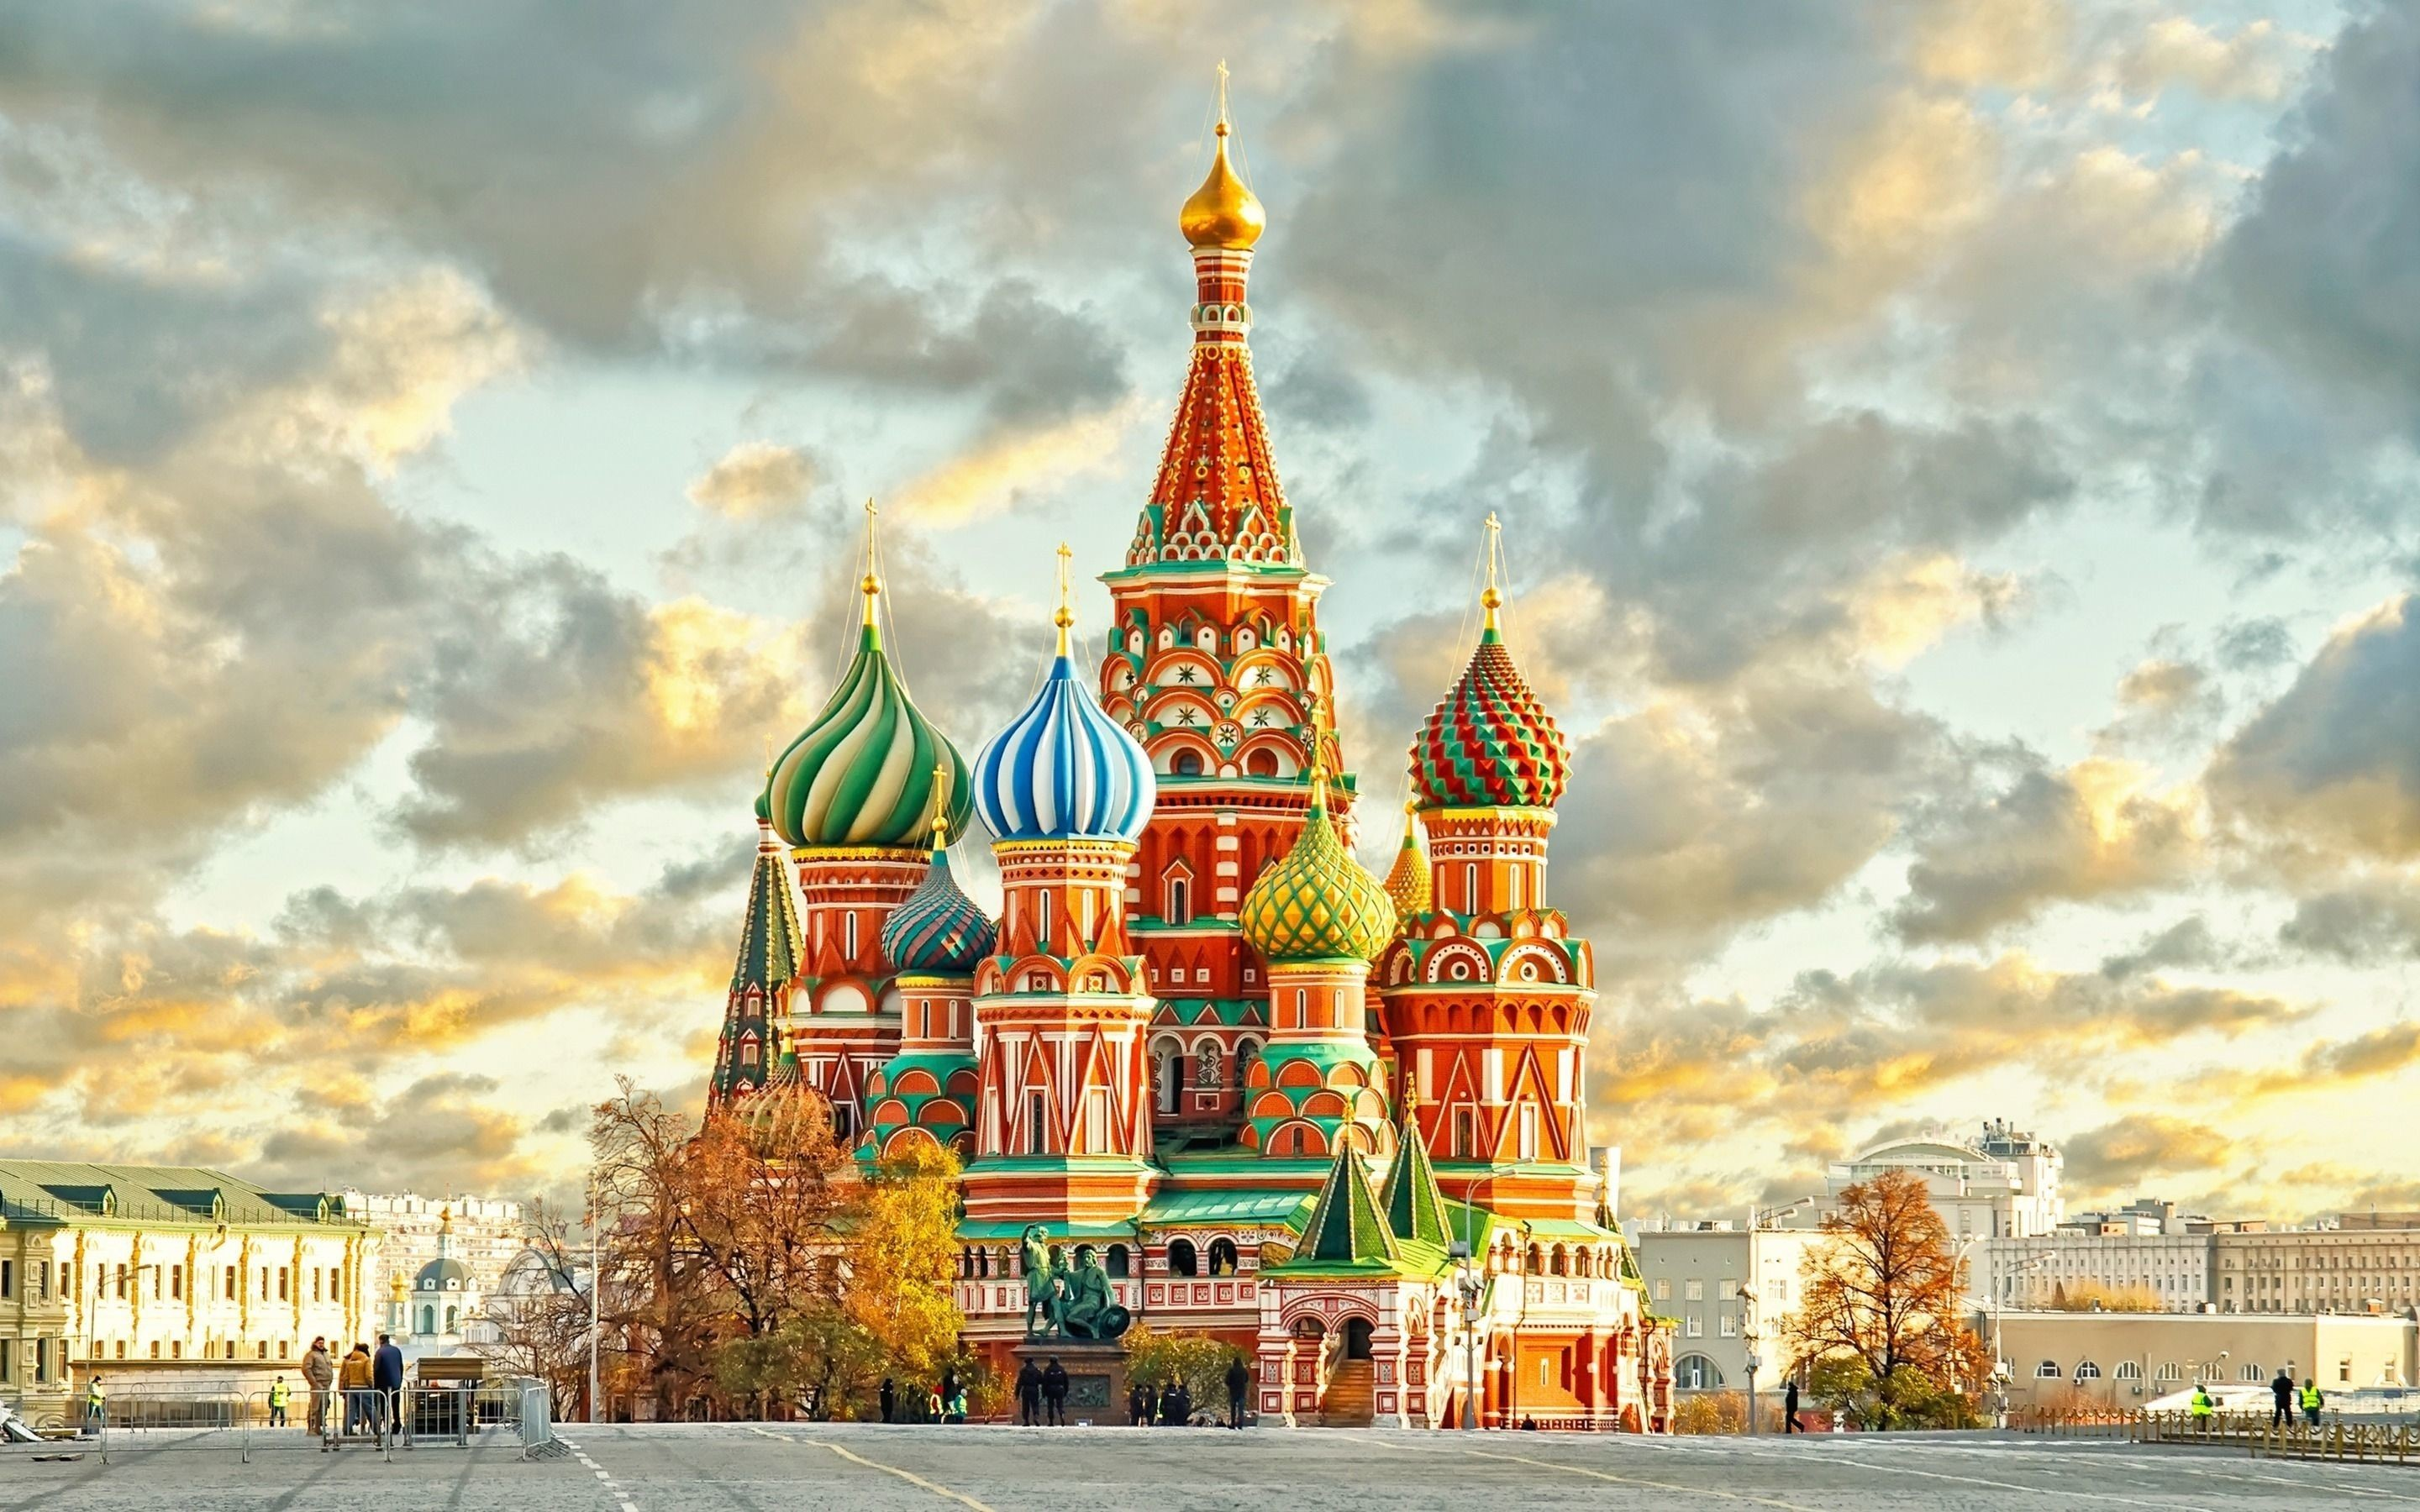
\includegraphics[height=4cm,width=5cm]{Moscow.jpg}	
		\label{Fig2.1}
		}
	\hspace*{1cm}
		\subfigure[Berlin]{
		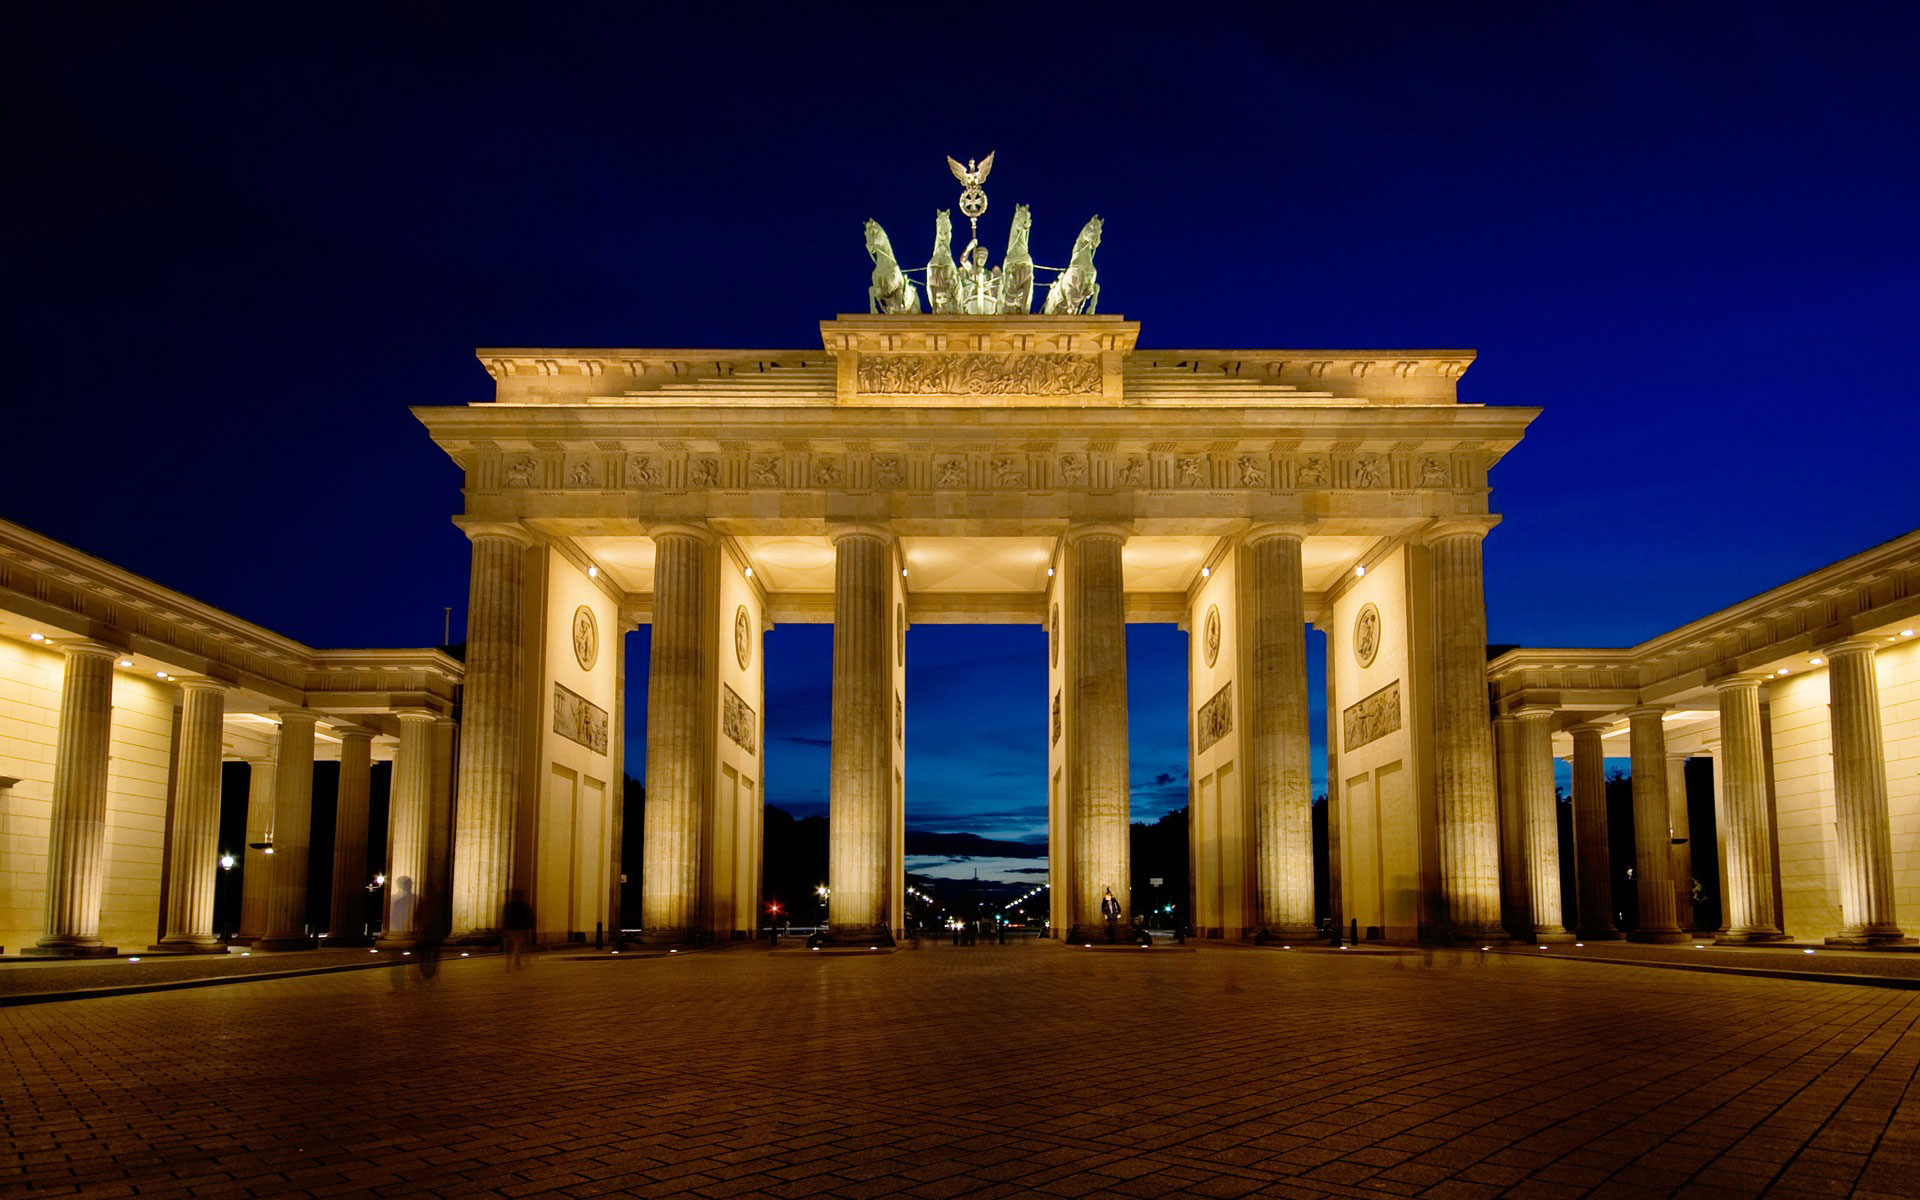
\includegraphics[height=4cm, width=5cm]{Berlin.jpg}
		\label{Fig2.2}
		}
	\end{center}

\end{figure}

سپس در تصویر \ref{Fig2.2}
می‌توان برلین را دید...




\end{document}